\section{Efficient Inference in Bayesian Networks}

\begin{frame} 

\mode<presentation>{
    \vspace{10mm}
    \begin{center} \huge
        \secname
    \end{center}
    
    \begin{itemize}
    \item a compact representation: turning DAG into a Junction tree,
    \item efficient Inference using message passing
    \end{itemize}
    }
\end{frame}

\begin{frame}

\begin{itemize}
\item \underline{Last time}:
\begin{itemize}
\item What is a graphical model
\item Performing inference using the full joint distribution
\item Product rule, Bayes' Theorem
\item exploiting conditional independence
\item Bayesian Networks (topology, cond. prob. tables)
\end{itemize}

\pause

\item \underline{Today}:
\begin{itemize}
\item the Junction tree algorithm
\item the message passsing algorithm (factor analysis anyone?)
\end{itemize}
\end{itemize}

\end{frame}

\subsection{Constructing Bayesian Networks}

\begin{frame} \frametitle{\subsubsecname}

	\begin{figure}[h]
		 \centering
		 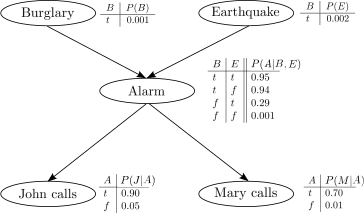
\includegraphics[width=0.5\textwidth]{img/section3_fig5_v2_2}%
		 \caption{DAG of the ``Californian'' example}
	\end{figure}
	
%	\only<2>{
%	\begin{itemize}
%		\item set of random variables 
%			$\leadsto$ nodes of the graph
%		\item direct influences between variables 
%			$\leadsto$ directed links between nodes
%		\item nodes $x_i$ are annotated with the conditional probabilities\\
%			\quad$P\big(X_i\,|\, \text{parents}(X_i)\big)$
%	\end{itemize}
%	} 
Considering statistical dependencies, only 10 instead of 31 entries have to be stored.
	{ \small
		\begin{align} 
			P(J,M,A,B,E) \stackrel{\substack{\text{product}\\\text{rule}}}{=}& 
			P(J|M,A,B,E) \, P(M|A,B,E) \, P(A|B,E) \, P(B|E) \, P(E) \\\slidesonly{\vspace{-5mm}}
			\stackrel{\substack{\text{cond.}\\\text{indep.}}}{=}& P(J|A) \, P(M|A) \, P(A|B,E) \, P(B) \, P(E)
		\end{align}
	}
\end{frame}

\begin{frame}\frametitle{\secname}
  
Bayesian Networks are a factorization of the full joint distribution\footnote{See Ch. 14 from \citep{russell2016artificial} for more details.}:

\begin{equation}
P(X_{1},\ldots,X_{n}) = \prod_{i=1}^{n} P(X_{i} | parents(X_{i}))
\end{equation}
    
\begin{itemize}
\item We only need to condition on the direct parents of any node $X_i$

\pause 
\item The factorization enables us to construct the \emph{directed acyclic graph} (DAG).
\item We can also use the DAG to formulate the factorization.
\end{itemize}

\begin{equation}
\mathit{DAG}_{\text{Bayes.Net}} \quad \corresponds \quad \prod_{i=1}^{n} P(X_{i} | parents(X_{i}))
\end{equation}
    
\end{frame}

\subsection{The Junction tree algorithm}

\begin{frame}\frametitle{\subsecname}

We need a representation that scales well for large DAGs to perform maginalisation (``summing out'') and conditioning more efficiently.

The Junction tree algorithm converts into a tree structure mad eup of \emph{cliques} and \emph{separators}.

\question{What is a difference between a DAG and a tree?}

\pause

- A tree structure guarantees that the path between any two nodes is unique.

\end{frame}

\begin{frame} \frametitle{Trees}
	\begin{itemize}
	\item\textbf{tree}: graph where each existing path 
			between nodes is \emph{unique}
	
	\vspace{2mm}
	\begin{center}
	\begin{tabular}{cc}
		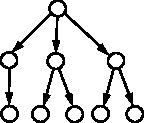
\includegraphics[width=4cm]{img/tree_directed}
		&
		\hspace{-5mm}
		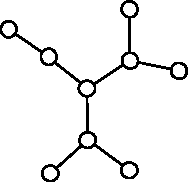
\includegraphics[width=5cm]{img/tree_undirected} \\
		directed tree & \hspace{-5mm} undirected tree 
	\end{tabular}
	\end{center}
	\end{itemize}
\end{frame}

\subsubsection{Overview of the Junction Tree algorithm}

\begin{frame}\frametitle{\subsubsecname}

\begin{align*}
\text{DAG}
\longrightarrow \substack{\text{moral}\\\text{graph}}
\longrightarrow \substack{\text{decomposable}\\\text{graph}}
\longrightarrow \substack{\text{bipartite}\\\text{graph}}
\longrightarrow \substack{\text{Junction}\\\text{Tree}}
\end{align*}

\end{frame}

\subsection{Decomposable Undirected Graphs}

\mode<presentation>{
\begin{frame} 
    \begin{center} \huge
        \secname
    \end{center}
    \begin{center}   
		\begin{align*}
		\text{DAG}
		\longrightarrow \substack{\text{moral}\\\text{graph}}
		\longrightarrow \substack{\text{\textcolor{blue}{decomposable}}\\\text{\textcolor{blue}{graph}}}
		\longrightarrow \substack{\text{bipartite}\\\text{graph}}
		\longrightarrow \substack{\text{Junction}\\\text{Tree}}
		\end{align*}
    \end{center}
\end{frame}
}

% -----------------------------------------------------------------------------
\begin{frame} \frametitle{Undirected Graph}
\begin{figure}
	\centering
	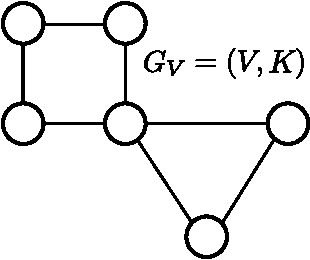
\includegraphics[width=4cm]{img/section3_fig9}
	 \caption{undirected graph $G_V$ with vertices $V$ and edges $K$} 
\end{figure}
\end{frame}

\mode<article>{
Separate $G$ (undirected graph) into two separate subgraphs $G_A$ and $G_B$
,
such that node $C$ lies on the path between \underline{any} node in $G_A$ and \underline{any} other node in $G_B$. 

\textbf{Remark}:
$C$ can also be a set of nodes (cf. ).
}

\subsubsection{Cliques and separators}

% -----------------------------------------------------------------------------
\begin{frame} \frametitle{Separators}

\only<1>{
\mode<presentation>{
	\begin{figure}
	\centering
	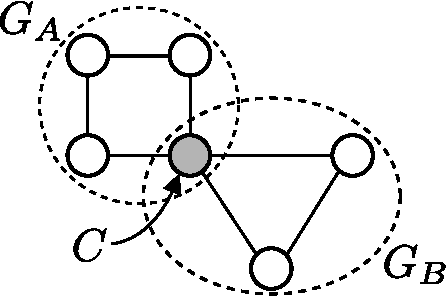
\includegraphics[width=5cm]{img/section3_fig10}
	\notesonly{\caption}\slidesonly{\caption*}{node C separates subsets A and B} 
	\end{figure}
}
}
\only<2>{
\begin{figure}[h]
     \centering
     \savebox{\imagebox}{
	 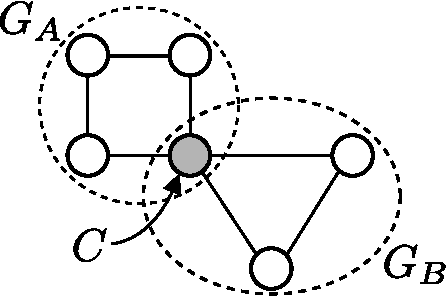
\includegraphics[width=0.45\textwidth]{img/section3_fig10}}%
     \begin{subfigure}[t]{0.35\textwidth}
         \centering
         \usebox{\imagebox}% Place largest image
         \caption{node C}
         \label{fig:nodes}
     \end{subfigure}
     \hspace{10mm}
     \begin{subfigure}[t]{0.45\textwidth}
         \centering
         \raisebox{\dimexpr.5\ht\imagebox-.5\height}{% Raise smaller image into place
         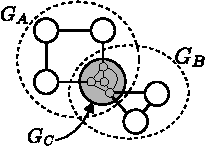
\includegraphics[width=0.99\textwidth]{img/section3_fig10_cset}
         }
         \caption{set of nodes C}
         \label{fig:setc}
     \end{subfigure}
     \caption{subsets A and B separated by C}
	 \label{fig:regression}
\end{figure}
}
	\slidesonly{\vspace{-2mm}}
	\begin{block}{Separator}
		A set $C$ of nodes \textbf{separates} two undirected subgraphs $G_A$ and $G_B$ 
		if \emph{every} path from node set $A$ to node set $B$ 
		has to pass through an element of $C$.
	\end{block}
\end{frame}


% -----------------------------------------------------------------------------
\begin{frame} \frametitle{Decomposable graphs}
	\vspace{-2mm}
	\begin{itemize}
		\item $A,B,C$ are a \textbf{proper decomposition} 
			of an undirected graph $G = (V,K)$ if:
			\vspace{0mm}
			\begin{itemize}
				\item $A,B,C$ are non-empty and 
					disjoint subsets with $V=A \cup B \cup C$,
				\item $C$ separates $G_A$ and $G_B$, and
				\item subgraph $G_C$ is complete.
			\end{itemize}
		\vspace{2mm}
		\item<2-> G is \textbf{decomposable} if it is complete, 
			or a proper decomposition $A,B,C$ exist,
			where $G_{A\cup C}$ and $G_{B \cup C}$ are decomposable.
	\end{itemize}
	\begin{center}
		\begin{tabular}{cc}
				\includegraphics<1-2>[height=3.75cm]{img/section3_fig12}
				\includegraphics<3>[height=3.75cm]{img/section3_fig13}
			& \visible<2->{
				\includegraphics<1-2>[height=3.75cm]{img/section3_fig12_v2}
				\includegraphics<3>[height=3.75cm]{img/section3_fig13_v2}
			}\\
				\only<1>{a proper decomposition}
				\only<2>{not a decomposable graph }
				\only<3>{a decomposable graph}
			& 
				\only<2>{$G_{A \cup C}$ is not decomposable}
				\only<3>{$G_{A \cup C}$ is decomposable and \\
            &   $G_{B \cup C}$ is complete}
		\end{tabular}
	\end{center}	
\end{frame}

